\documentclass[a4paper,11pt]{ltjsarticle}

% =============================================
% 1. パッケージ設定 (SARP v3.0 NNCT-EE準拠)
% =============================================
\usepackage[T1]{fontenc}
\usepackage{newtxtext}
\usepackage[varbb]{newtxmath} % 数式フォント Times系
\usepackage{bm}      % ベクトル太字
\usepackage{mathtools}

% レイアウト・図表関連
\usepackage[margin=25mm]{geometry}
\usepackage{array}      
\usepackage{multirow}   
\usepackage{fancyhdr}   
\usepackage{graphicx}
% 画像検索パス
\graphicspath{{./}{image/optimized/}{image/}}
\usepackage{float}
\usepackage{booktabs}
\usepackage{subcaption}
\usepackage{adjustbox}
\usepackage{placeins}

% 回路図・グラフ描画
\usepackage{circuitikz}
\usepackage{tikz}
\usepackage{pgfplots}
\pgfplotsset{compat=newest}
\usepackage{pgfplotstable}
\usetikzlibrary{arrows.meta, positioning, calc}

% SI単位・数式処理
\usepackage{siunitx}
\sisetup{
  detect-all,
  inter-unit-product=\ensuremath{{}\cdot{}},
  separate-uncertainty=true,
  number-unit-product = \hspace{0.5em} % 単位前の半角スペース強制
}

% リンク・参照
\usepackage{cite}
\usepackage[hidelinks]{hyperref}
\usepackage[nameinlink,noabbrev]{cleveref}
\usepackage{needspace}

% 参考文献の上付き表示設定 [1]形式
\makeatletter
\def\@cite#1#2{$^{\mbox{\scriptsize[#1\if@tempswa , #2\fi]}}$}
\def\@biblabel#1{[#1]}
\makeatother

\crefname{figure}{図}{図}
\crefname{table}{表}{表}
\crefname{equation}{式}{式}

% キャプション設定
\usepackage{caption}
\captionsetup{
  format=hang,
  labelsep=quad,
  font={small},
  labelfont={bf},
  justification=centering
}
\captionsetup[figure]{justification=centerlast}

% =============================================
% 2. カスタムコマンド定義
% =============================================
\newcommand{\UnderlineBox}[2][3cm]{\underline{\makebox[#1][c]{\vphantom{lp}\large #2}}}
\newcommand{\JustifiedLabel}[2]{\makebox[#1][s]{\large\bfseries #2}}
\newcommand{\BoldLabel}[1]{{\large\bfseries #1}}

% 微分記号(ローマン体 d)
\newcommand{\diff}[2]{\frac{\mathrm{d}#1}{\mathrm{d}#2}}
\newcommand{\pdiff}[2]{\frac{\partial #1}{\partial #2}}

% 単位記号・ローマン体コマンド(ショートカット)
% NOTE: Use siunitx's \si or \SI macros instead of defining a custom \unit to avoid conflicts with siunitx.
\newcommand{\rom}[1]{\mathrm{#1}}

% 箇条書き設定
\renewcommand{\labelenumi}{(\arabic{enumi})}

% =============================================
% 3. 表紙専用のページスタイル定義
% =============================================
\fancypagestyle{coverpage}{
  \fancyhf{} 
  \renewcommand{\headrulewidth}{0pt} 
  \renewcommand{\footrulewidth}{0pt} 
  \cfoot{\vspace{5mm}\Large \bfseries 国立長野高専 電気電子工学科}
}

% =============================================
% ドキュメント開始
% =============================================
\begin{document}

% /////////////////////////////////////////////
% 表紙 (Cover Page)
% /////////////////////////////////////////////

\newgeometry{top=25mm, bottom=20mm, left=18mm, right=18mm}
\thispagestyle{coverpage}

\begin{center}
    \vspace*{0mm} 
    {\Huge \bfseries 電気電子工学実験報告書}
    \vspace{10mm} 
\end{center}

\noindent
\begin{tabular}{@{}ll}
  \BoldLabel{テーマ名} & \UnderlineBox[13.5cm]{PCM通信} \\[2.0em] 
\end{tabular}

\noindent
\BoldLabel{報告者} \hspace{0.5em}
\UnderlineBox[1.5cm]{5} {\large \textbf{年}} \hspace{0.2em}      
(\UnderlineBox[1.5cm]{E} {\large \textbf{組}}) \hspace{0.2em} 
{\large \textbf{番号}} \UnderlineBox[2.0cm]{234} \hspace{0.5em}    
\UnderlineBox[1.5cm]{B} {\large \textbf{班}} \hspace{1em}        
\UnderlineBox[4.5cm]{栁原 魁人}                                   
\vspace{2.0em} 

\noindent
\begin{tabular}{@{}p{0.48\textwidth} p{0.48\textwidth}}
  \BoldLabel{実験場所} \hspace{1em} \UnderlineBox[5.5cm]{エレクトロニクス工房} & 
  \BoldLabel{指導担当} \hspace{1em} \UnderlineBox[5.5cm]{斎藤 栄輔}    
\end{tabular}
\vspace{2.0em} 

\noindent
\BoldLabel{共同実験者} \hspace{1em} \UnderlineBox[12.5cm]{石坂知尋,倉科純太郎,中井智大,中澤耕平} 
\vspace{2.5em} 

\noindent
\renewcommand{\arraystretch}{2.0}
\setlength{\tabcolsep}{0pt}
\begin{tabular}{l l l l}
    \JustifiedLabel{5em}{実験日} & 
    \hspace{0.3em} 令和 \UnderlineBox[0.65cm]{7} 年 \UnderlineBox[0.65cm]{9} 月 \UnderlineBox[0.65cm]{26} 日 & & \\
    \JustifiedLabel{5em}{提出期限} & 
    \hspace{0.3em} 令和 \UnderlineBox[0.65cm]{7} 年 \UnderlineBox[0.65cm]{12} 月 \UnderlineBox[0.65cm]{31} 日 & 
    \hspace{0.3em}$\Rightarrow$\hspace{0.3em} \JustifiedLabel{4em}{提出日} & 
    \hspace{0.3em} 令和 \UnderlineBox[0.65cm]{7} 年 \UnderlineBox[0.65cm]{12} 月 \UnderlineBox[0.65cm]{16} 日 \\
    ( \JustifiedLabel{6em}{再提出期限} & 
    \hspace{0.3em} 令和 \UnderlineBox[0.65cm]{} 年 \UnderlineBox[0.65cm]{} 月 \UnderlineBox[0.65cm]{} 日 & 
    \hspace{0.3em}$\Rightarrow$\hspace{0.3em} \JustifiedLabel{5em}{再提出日} & 
    \hspace{0.3em} 令和 \UnderlineBox[0.65cm]{} 年 \UnderlineBox[0.65cm]{} 月 \UnderlineBox[0.65cm]{} 日 ) \\
\end{tabular}
\vfill 

\renewcommand{\arraystretch}{1.5}
\begin{center}
\begin{tabular}{|>{\centering\arraybackslash}m{2.4cm}|>{\raggedright\arraybackslash}m{12.1cm}|>{\centering\arraybackslash}m{2.4cm}|}
\hline
\multicolumn{2}{|c|}{\JustifiedLabel{11em}{評 価 項 目}} & \JustifiedLabel{4em}{評 価} \\
\hline
\multirow{3}{*}{\parbox[c][4.5em][c]{2.4cm}{\centering\shortstack{\large\bfseries 実 習\\[0.3em]\large\bfseries 評 価}}} 
 & (1) 自ら積極的に実験に取り組めた &  \\ \cline{2-3}
 & (2) 実験装置を適切に使用でき,正確に実験を行なえた &  \\ \cline{2-3}
 & (3) グループ内で協力的に実験が行なえた &  \\
\hline
\multirow{4}{*}{\parbox[c][6.0em][c]{2.4cm}{\centering\shortstack{\large\bfseries 報告書\\[0.3em]\large\bfseries 評 価}}} 
 & (1) 結果のまとめかた(図表を含む) &  \\ \cline{2-3}
 & (2) 結果に対する考察 &  \\ \cline{2-3}
 & (3) 報告事項/課題(正しい解答や適切な引用など) &  \\ \cline{2-3}
 & (4) 報告書としての体裁が整っているか &  \\
\hline
\end{tabular}
\end{center}
\clearpage

% /////////////////////////////////////////////
% 本文 (Main Body)
% /////////////////////////////////////////////

\restoregeometry 
\setcounter{page}{1}
\pagestyle{plain} 

\section{目的}
パルス符号変復調(PCM: Pulse Code Modulation)は,アナログ信号をデジタル信号に変換して伝送する現代通信の基盤技術である.本実験では,回路シミュレータを用いることで,PCM変復調を構成する各機能ブロック(標本化,量子化,符号化,多重化,および復調)の回路動作を解析し,その基本原理と回路的実現手法を習得することを目的とした.

\section{原理}

\subsection{PCM通信システムの全体構成}
PCM方式は,連続的なアナログ信号を時間的および振幅的に離散化し,符号として伝送する方式である.図\ref{fig:1}にPCM通信の基本ブロック図を示す.
送信側(変調部)は以下の回路群より構成される.
\begin{itemize}
    \item \textbf{切換回路}: 複数の入力信号を時分割多重(TDM)するために順次選択する.
    \item \textbf{標本化回路}: 時間的に連続な信号を一定周期 $T_s$ でサンプリングし,標本値(PAM信号)を得る.
    \item \textbf{量子化・符号化回路}: 標本値を離散的なレベルに近似(量子化)し,2進デジタル信号へ変換(符号化)する.
\end{itemize}
受信側(復調部)では,分離回路によって同期信号や各チャンネル信号を分離し,D/A変換およびローパスフィルタ(LPF)を経て元のアナログ信号を復元する.

\begin{figure}[H]
  \centering
  \includegraphics[width=0.6\textwidth,height=0.45\textheight,keepaspectratio]{image/img_000.png}
  \caption{PCM通信の基本方式}
  \label{fig:1}
\end{figure}

\subsection{タイミングパルス発生回路}
システム全体の同期をとるためのパルス生成回路を図\ref{fig:2}に示す.
本回路は,カウンタIC (SN74LS162) とJKフリップフロップ (SN7476) を組み合わせた分周回路である.原発振クロック(\SI{125}{\kilo\hertz})をカウントし,所定のカウント値でキャリー出力 (RCO) を発生させる.このRCO信号をJKフリップフロップのクロック入力とすることで,トグル動作による分周波形(T1, T2など)を生成する.

\begin{figure}[H]
  \centering
  \includegraphics[width=0.75\textwidth,height=0.45\textheight,keepaspectratio]{image/img_001.png}
  \caption{タイミングパルス発生回路の回路図と真理値表}
  \label{fig:2}
\end{figure}

\begin{figure}[H]
  \centering
  \includegraphics[width=0.6\textwidth,height=0.45\textheight,keepaspectratio]{image/img_002.png}
  \caption{切換回路}
  \label{fig:3}
\end{figure}

\subsection{標本化回路(サンプル\&ホールド)}
図\ref{fig:4}に標本化回路を示す.アナログスイッチ (SW1) とコンデンサ (C1),およびボルテージフォロワ(OP1)により構成される.
サンプリングパルス (Clock) がHighの期間,SW1が閉じてC1が入力電圧まで充電される(サンプルモード).ClockがLowになるとSW1が開き,C1の電荷はオペアンプの高入力インピーダンスにより保持される(ホールドモード).これにより,A/D変換に必要な一定電圧期間を生成する.

\begin{figure}[H]
  \centering
  \includegraphics[width=0.7\textwidth,height=0.45\textheight,keepaspectratio]{image/img_003.png}
  \caption{標本化回路(サンプル\&ホールド回路)}
  \label{fig:4}
\end{figure}

\subsection{波形合成・分離回路}
多重化伝送における信号合成と分離の原理モデルを図\ref{fig:7}に示す.
合成側では,演算増幅器を用いた加算回路により,異なるタイミングパルス(T2, T3)を加算して多値波形 (Vmix) を生成する.
分離側では,理想ダイオードの整流作用と反転増幅器の閾値特性を利用し,電圧レベルに応じて信号経路を切り替えることで元のパルスを分離する.

\begin{figure}[H]
  \centering
  \includegraphics[width=0.7\textwidth,height=0.45\textheight,keepaspectratio]{image/img_006.png}
  \caption{波形合成・分離回路}
  \label{fig:7}
\end{figure}

\begin{figure}[H]
  \centering
  \includegraphics[width=0.6\textwidth,height=0.45\textheight,keepaspectratio]{image/img_007.png}
  \caption{波形合成・分離回路の動作原理}
  \label{fig:8}
\end{figure}

\begin{figure}[H]
  \centering
  \includegraphics[width=0.7\textwidth,height=0.45\textheight,keepaspectratio]{image/img_008.png}
  \caption{AD・DA変換回路とローパスフィルタ}
  \label{fig:9}
\end{figure}

\FloatBarrier

\section{実験方法}
本実験では,回路シミュレーションソフトウェア **TINA-TI** (Texas Instruments) を使用し,以下の手順で回路動作の検証を行った.

\begin{enumerate}
    \item **タイミングパルス発生回路の構築**: 
    図\ref{fig:2}に示す回路を作成し,マクロ(サブサーキット)として登録した(図\ref{fig:10}).これにより,大規模な回路におけるクロック源としての再利用を可能とした.

    \begin{figure}[H]
      \centering
      \includegraphics[width=0.7\textwidth,height=0.45\textheight,keepaspectratio]{image/img_009.png}
      \caption{タイミングパルス発生回路のマクロ化}
      \label{fig:10}
    \end{figure}
    
    \item **各機能ブロックの過渡解析**:
    以下の各回路についてシミュレーション回路を構築し,過渡解析 (Transient Analysis) を実行した.
    \begin{itemize}
        \item 切換回路(図\ref{fig:3})
        \item 標本化回路(図\ref{fig:4})
        \item シフトレジスタ(図\ref{fig:6})
        \item 波形合成・分離回路(図\ref{fig:7})
        \item AD-DA変換およびLPF回路(図\ref{fig:9})
    \end{itemize}

    \item **パラメータ検証**: 
    標本化回路におけるダミー抵抗 $R_1$ の有無による影響や,シフトレジスタの入力スイッチ設定による出力波形の変化を確認した.
\end{enumerate}


\section{使用機器}
本実験で使用した環境を表\ref{tab:equipment}に示す.

\begin{table}[H]
\caption{使用機器およびソフトウェア}
\label{tab:equipment}
\centering
\begin{tabular}{ll}
\toprule
\textbf{種別} & \textbf{名称・仕様} \\
\midrule
ソフトウェア & TINA-TI (SPICE-Based Analog Simulation Program) \\
開発元 & DesignSoft / Texas Instruments \\
OS & Microsoft Windows 10 Education \\
\bottomrule
\end{tabular}
\end{table}

\section{結果および考察}

\subsection{タイミングパルス発生回路}
タイミングパルス発生回路のシミュレーション結果を図\ref{fig:11}に示す.
クロック信号 (clock) の入力に対し,カウンタ出力 (RCO) が周期的に発生している.これに同期して,JKフリップフロップの出力 (T1, T2) が反転動作を繰り返していることが確認できる.T1の周波数はclockの周波数に対して分周されており,回路が正常な分周器およびタイミングジェネレータとして機能していることが確認された.

\begin{figure}[H]
  \centering
  \includegraphics[width=0.75\textwidth,height=0.45\textheight,keepaspectratio]{image/img_010.png}
  \caption{タイミングパルス発生回路の出力波形}
  \label{fig:11}
\end{figure}

\subsection{標本化回路}
標本化回路の動作波形を図\ref{fig:13}に示す.
緑色のパルス (Vclock) がHighの区間において,赤色の出力電圧 (Vout) は入力正弦波 (VG1) に追従している.一方,VclockがLowの区間では,直前の電圧値が水平に保持されている.
これは,原理で述べた「コンデンサへの充電」と「高インピーダンスによる電荷保持」が理想的に行われていることを示している.なお,シミュレーション上ではオペアンプの入力電流が無視できるほど小さいため,電圧降下(ドループ)は観測されず,理想的なサンプル\&ホールド特性が得られた.

\begin{figure}[H]
  \centering
  \includegraphics[width=0.75\textwidth,height=0.45\textheight,keepaspectratio]{image/img_012.png}
  \caption{標本化回路の入出力波形}
  \label{fig:13}
\end{figure}

\subsection{波形合成・分離回路}
図\ref{fig:15}に波形合成・分離回路の解析結果を示す.
合成波形 (Vmix) は,正のパルス (T2由来) と負のパルス (T3由来) が時間軸上で重畳された波形となっている.
これに対し,分離回路の出力 VT2 および VT3 を確認すると,Vmix からそれぞれの成分のみが正のパルスとして抽出されている.これは,図\ref{fig:7}および図\ref{fig:8}で示したダイオードロジックによる電圧選別機能が,理論通りに動作していることを実証するものである.

\begin{figure}[H]
  \centering
  \includegraphics[width=0.75\textwidth,height=0.45\textheight,keepaspectratio]{image/img_014.png}
  \caption{波形合成・分離回路の各部波形}
  \label{fig:15}
\end{figure}

\subsection{AD-DA変換および復調回路}
システム全体の動作を示すAD-DA変換・復調回路の結果を図\ref{fig:16}に示す.
\begin{enumerate}
    \item \textbf{A/D変換}: 入力信号 (Vin) に応じて,デジタルデータ (VQA, VQHなど) が変化しており,量子化が正常に行われている.
    \item \textbf{D/A変換}: VDA波形は階段状の波形となっており,離散的な電圧レベルが出力されている.これはゼロ次ホールド特性を持つD/A変換の典型的な挙動である.
    \item \textbf{復調}: 最終段のLPF出力 (V復調) は,VDAの急峻な変化(高周波成分)が除去され,滑らかな正弦波に復元されている.
\end{enumerate}
入力信号 (VG1) と比較すると,位相遅れが生じているものの,波形歪みは小さく,適切に復調されているといえる.位相遅れはLPFの群遅延特性に起因するものであり,回路構成上妥当な結果である.

\begin{figure}[H]
  \centering
  \includegraphics[width=0.75\textwidth,height=0.45\textheight,keepaspectratio]{image/img_015.png}
  \caption{AD-DA変換およびLPF通過後の復調波形}
  \label{fig:16}
\end{figure}

\section{報告事項}

\subsection{標本化定理(サンプリング定理)}
アナログ信号をデジタル処理するために離散化する際,元の信号情報を損なわずに標本化するための条件を定めたものが標本化定理である.
帯域制限された信号の最大周波数を $f_{max}$ とするとき,標本化周波数 $f_s$ は次式を満たす必要がある.
\begin{equation}
  f_s \ge 2 f_{max}
\end{equation}
この条件が満たされない場合,元の信号スペクトルと折り返しスペクトル(エイリアシング成分)が重なり合い,元の波形を復元することが不可能となる.復元には,遮断周波数 $f_c$ ($f_{max} < f_c < f_s - f_{max}$) の理想的な低域通過フィルタを用いる.

\subsection{量子化雑音とSN比}
量子化とは,連続的な振幅値を離散的な値に丸める処理であり,この際に生じる誤差を量子化雑音という.
$n$ ビットの直線量子化において,信号対量子化雑音比 (SNR) は以下の理論式で与えられる\texorpdfstring{\cite{hatori2012}}{}.
\begin{equation}
  SNR \, [\si{\decibel}] = 6.02 n + 1.76
\end{equation}
本実験では $n=8$ ビットであるため,理論上の最大SNRは,
\begin{equation}
  SNR = 6.02 \times 8 + 1.76 \approx \SI{49.9}{\decibel}
\end{equation}
となる.

\subsection{サレン・キー型LPFの周波数特性}
実験で使用したローパスフィルタ(図\ref{fig:19}参照)は,サレン・キー (Sallen-Key) 型と呼ばれる2次アクティブフィルタである.オペアンプをボルテージフォロワ(利得 $K=1$)として使用した場合の伝達関数 $G(s)$ は次式で表される\texorpdfstring{\cite{ti_sallen_key}}{}.

\begin{figure}[H]
  \centering
  \includegraphics[width=0.7\textwidth,height=0.45\textheight,keepaspectratio]{image/img_017.png}
  \caption{サレン・キー型アクティブローパスフィルタ(LPF)}
  \label{fig:19}
\end{figure}

\begin{equation}
  G(s) = \frac{1}{s^2 C_1 C_2 R_1 R_2 + s C_2 (R_1 + R_2) + 1}
\end{equation}
ここで,実験回路定数 $R_1 = R_2 = R = \SI{50}{\kilo\ohm}$,$C_1 = \SI{2.3}{\nano\farad}$,$C_2 = \SI{1.1}{\nano\farad}$ を代入すると,遮断周波数 $f_c$ は以下のように計算される.
\begin{equation}
  f_c = \frac{1}{2\pi \sqrt{R_1 R_2 C_1 C_2}} = \frac{1}{2\pi R \sqrt{C_1 C_2}} \approx \SI{2001}{\hertz}
\end{equation}
図\ref{fig:lpf_bode}に,この伝達関数に基づく理論周波数特性(ボード線図)を示す.\SI{2}{\kilo\hertz} 付近から利得が減少し始め,-40 dB/dec の傾きで減衰する特性が確認できる.

\begin{figure}[H]
  \centering
  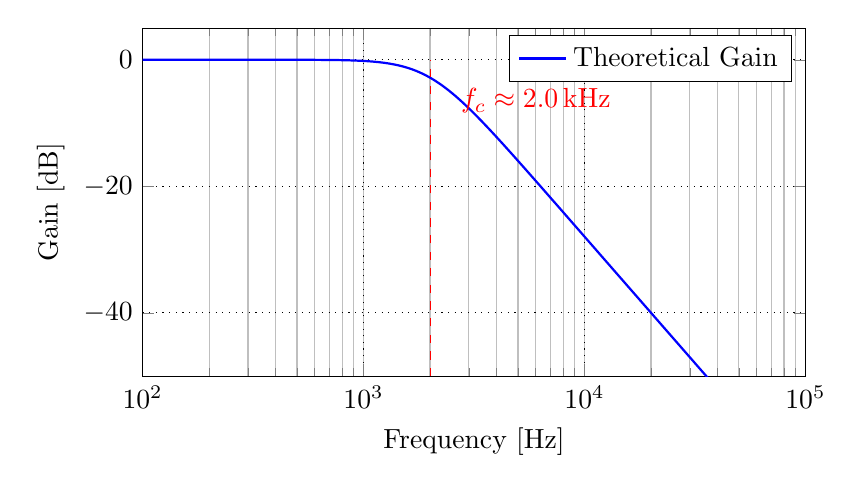
\begin{tikzpicture}
    \begin{semilogxaxis}[
        width=10cm, height=6cm,
        xlabel={Frequency [\si{\hertz}]},
        ylabel={Gain [\si{\decibel}]}, 
        grid=both,
        major grid style={dotted,black},
        xmin=100, xmax=100000,
        ymin=-50, ymax=5,
      ]
      % fc = 2001 Hz, Q = 0.723
      \addplot[thick, blue, domain=100:100000, samples=200] {20*log10( 1 / sqrt( (1-(x/2001)^2)^2 + ( (x/2001)/0.723 )^2 ) ) };
      \addlegendentry{Theoretical Gain}
      \draw[dashed, red] (axis cs: 2001, -50) -- (axis cs: 2001, 0);
      \node[red, anchor=south west] at (axis cs: 2500, -10) {$f_c \approx \SI{2.0}{\kilo\hertz}$};
    \end{semilogxaxis}
  \end{tikzpicture}
  \caption{サレン・キー型LPFの理論周波数特性}
  \label{fig:lpf_bode}
\end{figure}

\section{参考文献}
\begin{thebibliography}{99}
    \bibitem{kaneko1977_1} 金子尚志:「PCM 通信の技術」,産報出版株式会社,pp.17-19 (1977).
    \bibitem{hatori2012} 羽鳥光俊:「わかりやすい通信工学」,コロナ社,p.21 (2012).
    \bibitem{takasaki2021} 高崎和之:「基本からわかる電子回路」,株式会社ナツメ社,pp.36-37 (2021).
    \bibitem{ti_sallen_key} Texas Instruments: "Analysis of the Sallen-Key Architecture (Rev. B)", \url{https://www.ti.com/lit/an/sloa024b/sloa024b.pdf} (参照 2025-12-16).
\end{thebibliography}

\end{document}